\documentclass[12pt,letterpaper]{article}
\usepackage[utf8]{inputenc}
\usepackage[T1]{fontenc}
\usepackage[spanish,es-nodecimaldot]{babel}
\usepackage{graphicx}
\usepackage{geometry}
\usepackage{tikz} 

% --- PAQUETES PARA CÓDIGO FUENTE ---
\usepackage{listings}
\usepackage{xcolor}

% --- PAQUETE PARA HIPERVÍNCULOS ---
\usepackage[colorlinks=true, linkcolor=blue, urlcolor=blue, citecolor=blue]{hyperref}

% Definición de colores estilo editor
\definecolor{fondo}{rgb}{0.95, 0.95, 0.96}
\definecolor{comentarios}{rgb}{0.0, 0.5, 0.0}
\definecolor{palabrasclave}{rgb}{0.0, 0.0, 0.8}
\definecolor{cadenas}{rgb}{0.6, 0.1, 0.1}
\definecolor{numeros}{rgb}{0.5, 0.5, 0.5}

% --- ENSEÑARLE RUST A LATEX ---
\lstdefinelanguage{Rust}{
  keywords={fn, let, mut, for, in, if, else, return, pub, struct, impl, enum, match, use, mod, const, static, vec, f64, u32, i32, Vec, String},
  sensitive=true,
  comment=[l]{//},
  morecomment=[s]{/*}{*/},
  morestring=[b]",
  morestring=[b]'
}

% Configuración global del entorno de código
\lstdefinestyle{estilocodigo}{
    backgroundcolor=\color{fondo},   
    commentstyle=\color{comentarios},
    keywordstyle=\bfseries\color{palabrasclave},
    stringstyle=\color{cadenas},
    numberstyle=\tiny\color{numeros},
    basicstyle=\ttfamily\footnotesize,
    breakatwhitespace=false,         
    breaklines=true,                 
    captionpos=b,                    
    keepspaces=true,                 
    numbers=left,                    
    numbersep=10pt,                  
    showspaces=false,                
    showstringspaces=false,
    showtabs=false,                  
    tabsize=4,
    frame=single, 
    rulecolor=\color{lightgray}
}
\lstset{style=estilocodigo}

% Márgenes formales
\geometry{
    top=3cm,
    bottom=3cm,
    left=3cm,
    right=3cm
}

\begin{document}

\begin{titlepage}
    \centering

    % --- ENCABEZADO: LOGOS E INSTITUCIÓN ---
    \begin{minipage}{0.15\textwidth}
        \begin{flushleft}
            
\includegraphics[height=3cm, keepaspectratio]{ipn_logo.png}
        \end{flushleft}
    \end{minipage}
    \hfill
    \begin{minipage}{0.65\textwidth}
        \centering
        {\large \textbf{INSTITUTO POLITÉCNICO NACIONAL}}\\[0.3cm]
        {\large \textbf{ESCUELA SUPERIOR DE FÍSICA Y MATEMÁTICAS}}
    \end{minipage}
    \hfill
    \begin{minipage}{0.15\textwidth}
        \begin{flushright}
            
\includegraphics[height=3cm, keepaspectratio]{esfm_logo.jpg}
        \end{flushright}
    \end{minipage}

    \vspace{1cm}
    \rule{\linewidth}{1.5pt} 
    \vspace{2cm}

    % --- CARRERA Y MATERIA ---
    {\Large \textbf{Licenciatura en Matemáticas Algorítmicas}} \\[1.5cm]
    {\large Unidad de Aprendizaje:} \\[0.2cm]
    {\LARGE \textbf{Análisis Matemático}} \\[2.5cm]

    % --- TÍTULO DEL TRABAJO ---
    {\Huge \textbf{Conjunto de Cantor}} \\[3cm]

    % --- AUTOR ---
    {\large \textbf{Alumno:}} \\[0.3cm]
    {\Large Joel Reyes Garcia} \\[2cm]

    \vfill

    % --- LUGAR Y FECHA ---
    {\large Ciudad de México} \\
    \vspace{0.3cm}
    {\large \today}

\end{titlepage}

% =========================================================
% --- SECCIÓN DE CÓDIGO ---
% =========================================================
\newpage
\section*{Cálculo Algorítmico del Conjunto}

Cuando empecé a modelar el Conjunto de Cantor, me di cuenta rápido de que el problema real no era dibujar las líneas, sino manejar la memoria. Como la cantidad de segmentos crece con una complejidad espacial de $\mathcal{O}(2^n)$, Python se quedaba sin recursos o se volvía muy lento al calcular millones de intervalos. Por eso decidí hacer el cálculo pesado en Rust. Rust es excelente manejando la memoria de forma eficiente, lo cual era justo lo que necesitaba para este algoritmo. 

Para no complicarme demasiado conectando ambos lenguajes, utilicé \texttt{maturin} y \texttt{PyO3}. Estas herramientas me permitieron escribir mi función matemática en Rust, compilarla fácilmente y luego importarla en Python como si fuera una librería normal. Así, Rust hace todo el trabajo duro de calcular las coordenadas, y Python solo se encarga de lo que hace mejor: dibujar y mostrar la interfaz al usuario.

\vspace{0.5cm}

\begin{lstlisting}[language=Rust, caption=Cálculo del Conjunto de Cantor optimizado en memoria usando Rust]
use pyo3::prelude::*;

#[pyfunction]
fn conjunto_de_cantor(iteraciones: u32) -> PyResult<Vec<(f64, f64)>> {
    let mut intervalos = vec![(0.0, 1.0)];

    for _ in 0..iteraciones {
        let mut nuevos_intervalos = Vec::with_capacity(intervalos.len() * 2);
        
        for (inicio, fin) in intervalos {
            let distancia = (fin - inicio) / 3.0;
            
            nuevos_intervalos.push((inicio, inicio + distancia));
            nuevos_intervalos.push((fin - distancia, fin));
        }
        intervalos = nuevos_intervalos;
    }

    Ok(intervalos)
}

#[pymodule]
fn CantorLib(m: &Bound<'_, PyModule>) -> PyResult<()> {
    m.add_function(wrap_pyfunction!(conjunto_de_cantor, m)?)?;
    Ok(())
}
\end{lstlisting}

En el código, usé un tipo \texttt{u32} (entero sin signo) para las iteraciones porque, matemáticamente, no vamos a pedir iteraciones negativas, y mi computadora saturaría su memoria RAM mucho antes de llegar al límite de ese número. Lo que sí era vital era usar flotantes de 64 bits (\texttt{f64}) para guardar los intervalos. 

El mayor truco de optimización que implementé fue \texttt{Vec::with\_capacity}. En lugar de dejar que el programa adivinara cuánta memoria iba a necesitar y perdiera tiempo reasignando arreglos, le digo exactamente cuánto espacio reservar desde el inicio de cada paso (exactamente el doble del vector anterior). Después, solo es cuestión de tomar cada segmento, calcular la distancia dividiendo su longitud entre 3, y guardar las nuevas coordenadas de los extremos izquierdo y derecho (ver Figura 1).

\begin{figure}[htpb]
    \centering
    \begin{tikzpicture}[x=12cm, y=1cm]
        % Eje central invisible para alinear
        \draw[draw=none] (0, 0.5) -- (1, 0.5);
        
        % Iteración 0
        \draw[ultra thick, color=black] (0, 0) -- (1, 0) node[right, xshift=15pt] {$n=0$};
        \node[above] at (0, 0) {\small $0.0$};
        \node[above] at (1, 0) {\small $1.0$};
        
        % Iteración 1
        \draw[ultra thick, color=black] (0, -1) -- (1/3, -1);
        \draw[ultra thick, color=black] (2/3, -1) -- (1, -1) node[right, xshift=15pt] {$n=1$};
        \node[below] at (1/3, -1) {\small $1/3$};
        \node[below] at (2/3, -1) {\small $2/3$};
        
        % Iteración 2
        \draw[ultra thick, color=black] (0, -2) -- (1/9, -2);
        \draw[ultra thick, color=black] (2/9, -2) -- (1/3, -2);
        \draw[ultra thick, color=black] (2/3, -2) -- (7/9, -2);
        \draw[ultra thick, color=black] (8/9, -2) -- (1, -2) node[right, xshift=15pt] {$n=2$};
        
    \end{tikzpicture}
    \vspace{0.3cm}
    \caption{Representación gráfica de la división matemática programada en el ciclo de Rust.}
\end{figure}

\section*{Visualización e Interfaz}

Con la matemática resuelta, el script de Python importa la librería \texttt{CantorLib.so} recién compilada. Agregué un \texttt{input} sencillo para que el usuario elija hasta qué nivel del fractal quiere profundizar. Luego, meto esos datos en arreglos de \texttt{NumPy} para manejarlos en bloque y uso \texttt{Matplotlib} para pintarlos en pantalla.

\vspace{0.5cm}

\begin{lstlisting}[language=Python, caption=Interfaz de ejecución y renderizado vectorial en Python]
import os
import sys
import time
import subprocess
import shutil
import importlib.util
import math
import numpy as np
import matplotlib.pyplot as plt
from matplotlib.collections import LineCollection

if os.path.exists("CantorLib/Cargo.toml"):
    try:
        subprocess.check_call(
            ["cargo", "build", "--release"], 
            cwd="CantorLib", stdout=subprocess.DEVNULL, stderr=subprocess.STDOUT
        )
        shutil.copy("CantorLib/target/release/libCantorLib.so", "CantorLib.so")
    except Exception as e:
        if not os.path.exists("CantorLib.so"): sys.exit(1)

ruta_so = os.path.abspath("CantorLib.so")
spec = importlib.util.spec_from_file_location("CantorLib", ruta_so)
CantorLib = importlib.util.module_from_spec(spec)
sys.modules["CantorLib"] = CantorLib
spec.loader.exec_module(CantorLib)

ITERACIONES = int(input('Elige el numero de iteraciones: \n'))

t0 = time.time()
segs_por_nivel = []
for i in range(ITERACIONES + 1):
    inter = CantorLib.conjunto_de_cantor(i)
    segs_por_nivel.append(np.array(inter, dtype=np.float64))

print(f"Calculados {2**(ITERACIONES+1)-1:,} elementos en {time.time() - t0:.3f}s")

fig, ax = plt.subplots(figsize=(12, 8))
coleccion = LineCollection([], colors='black', linewidths=8.0, antialiased=False)
coleccion.set_capstyle('butt')
ax.add_collection(coleccion)

def actualizar_escena(event_ax=None):
    for txt in list(ax.texts):
        txt.remove()

    xlim = ax.get_xlim()
    ancho_vista = xlim[1] - xlim[0]
    
    if ancho_vista <= 0: return
    
    min_dx = ancho_vista / 1920.0 
    
    try:
        j_max = int(math.log(1.0 / min_dx) / math.log(3.0)) + 1
    except ValueError:
        j_max = ITERACIONES

    segs_a_dibujar = []

    for i in range(ITERACIONES + 1):
        k = min(i, j_max, ITERACIONES)
        segs_k = segs_por_nivel[k]
        
        mask = (segs_k[:, 1] >= xlim[0]) & (segs_k[:, 0] <= xlim[1])
        visibles = segs_k[mask]
        
        if len(visibles) > 0:
            n_vis = len(visibles)
            y_val = -i
            
            bloque = np.empty((n_vis, 2, 2))
            bloque[:, 0, 0] = visibles[:, 0]
            bloque[:, 0, 1] = y_val
            bloque[:, 1, 0] = visibles[:, 1]
            bloque[:, 1, 1] = y_val
            
            segs_a_dibujar.append(bloque)
            
            if i <= j_max:
                for x0, x1 in visibles:
                    dx_real = x1 - x0
                    if dx_real > (ancho_vista * 0.15):
                        caja_inicio = dict(boxstyle="round,pad=0.2", facecolor="#f4f8fa", edgecolor="#0055aa", alpha=0.9)
                        caja_fin = dict(boxstyle="round,pad=0.2", facecolor="#faf4f4", edgecolor="#aa0000", alpha=0.9)
                        
                        ax.annotate(f"{x0:.16g}", xy=(x0, y_val), xytext=(5, 18),
                                    textcoords="offset points", ha='left', va='bottom',
                                    fontsize=9, family='monospace', color='#003366',
                                    bbox=caja_inicio, arrowprops=dict(arrowstyle="->", color="#0055aa", shrinkB=4))
                        
                        ax.annotate(f"{x1:.16g}", xy=(x1, y_val), xytext=(-5, -18),
                                    textcoords="offset points", ha='right', va='top',
                                    fontsize=9, family='monospace', color='#660000',
                                    bbox=caja_fin, arrowprops=dict(arrowstyle="->", color="#aa0000", shrinkB=4))
            
    if segs_a_dibujar:
        coleccion.set_segments(np.vstack(segs_a_dibujar))
    else:
        coleccion.set_segments([])

    if event_ax:
        ax.figure.canvas.draw_idle()

ax.callbacks.connect('xlim_changed', actualizar_escena)

ax.set_xlim(-0.05, 1.05)
ax.set_ylim(-ITERACIONES - 1, 1)
ax.axis('off')
plt.title(f"Conjunto de Cantor - {ITERACIONES} Iteraciones\n", fontsize=14)
plt.tight_layout()

actualizar_escena()

plt.show()
\end{lstlisting}

\section*{Resultados y Rendimiento}

Los resultados confirman que delegar el cálculo algorítmico a Rust fue una excelente decisión. El programa calcula $2,097,151$ elementos en apenas $0.633$ segundos. Estos cálculos los realicé pidiendo $20$ iteraciones al sistema, que es el número recomendado para ver la complejidad del fractal sin quedarme sin memoria RAM.

\begin{figure}[htpb]
    \centering
    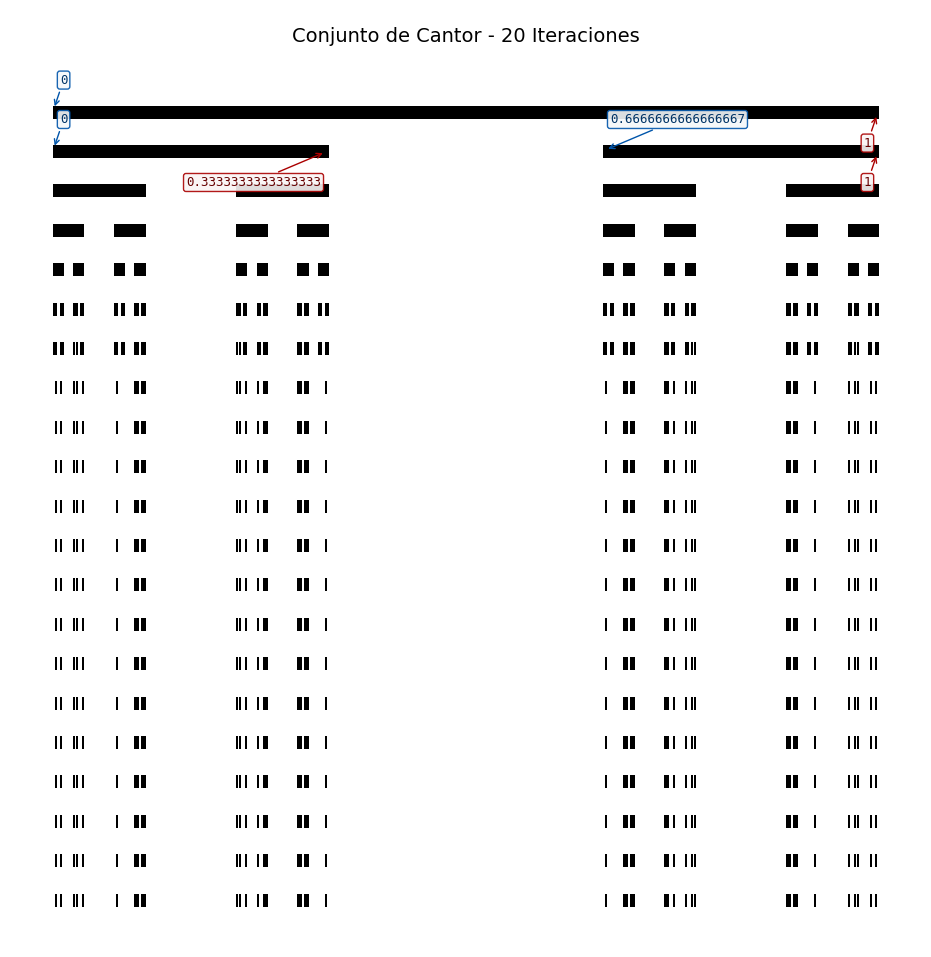
\includegraphics[width=0.9\textwidth]{output.png}
    \caption{Vista general del Conjunto de Cantor. En pocos milisegundos se despliegan más de dos millones de segmentos en pantalla.}
\end{figure}

Si miramos la gráfica sin acercarnos (Figura 2), parece que los segmentos simplemente se unen en líneas sólidas debido a los píxeles de la pantalla. Pero la precisión matemática está ahí. Al hacer zoom en la gráfica, el sistema vuelve a calcular qué partes estamos viendo y renderiza las coordenadas sin ningún tipo de retraso, probando que no se perdió ni un solo decimal en las profundidades del fractal (Figura 3).

\begin{figure}[htpb]
    \centering
    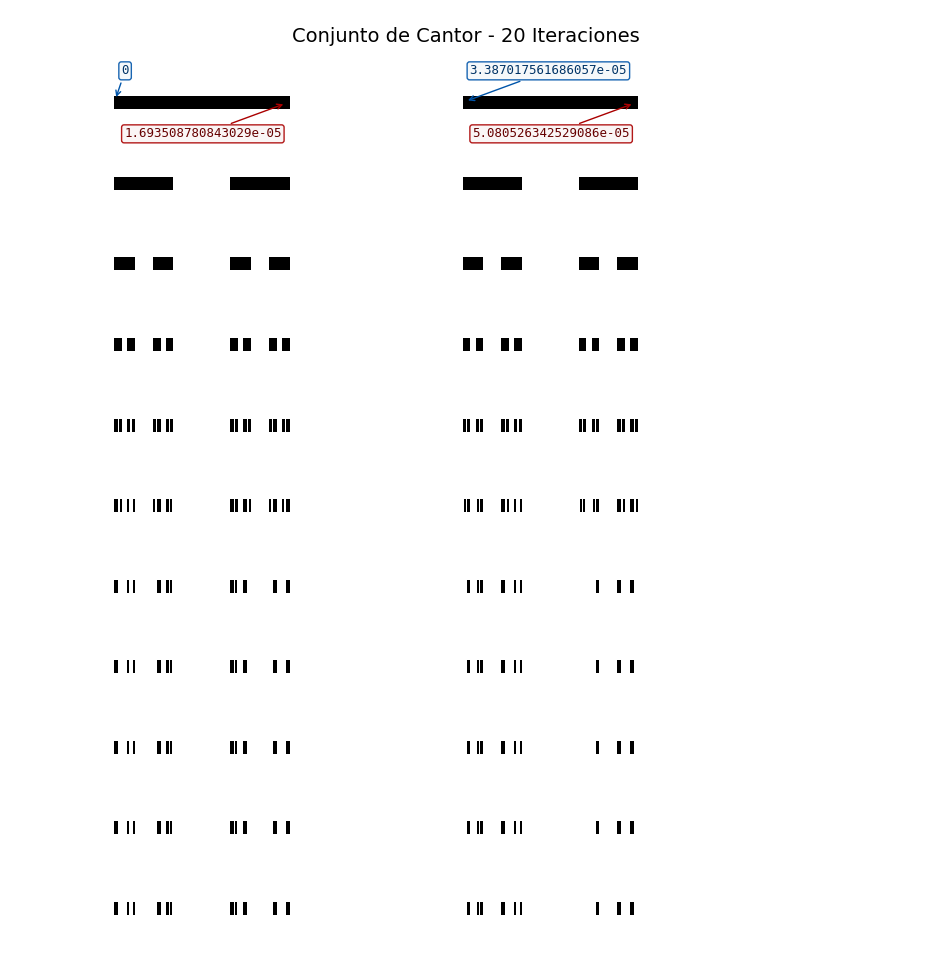
\includegraphics[width=0.9\textwidth]{output_1.png}
    \caption{Detalle de las coordenadas al hacer zoom. Los subsegmentos se definen perfectamente gracias al cálculo en f64.}
\end{figure}

% Forzar a LaTeX a vaciar la cola de imágenes antes de continuar
\clearpage

% --- SECCIÓN DE REPOSITORIO Y QR ---
\vspace*{\fill}
\begin{center}
    {\Large \textbf{Repositorio del Proyecto}} \\[0.4cm]
    El código fuente completo de esta implementación está disponible en GitHub: \\[0.3cm]
    \url{https://github.com/Jowl0/Conjunto_De_Cantor} \\[0.8cm]
    
\includegraphics[width=0.25\textwidth]{qr.png}
\end{center}
\vspace*{\fill}

\end{document}